\documentclass[../portafolio.tex]{subfiles}
\begin{document}
\section{Resultados}

\begin{enumerate}
\item \textbf{Primera Simulación}: 
Los datos obtenidos de esta simulación son representados en la tabla \ref{tab: tabla1}
  \\
   \\
   \begin{table}[]
     
    \begin{tabular}{|l|c|c|c|c|}\hline 
    \diagbox{Grosor(nm)}{Particulas (mol)} & 50 (mol) & 100 (mol) & 150 (mol) & \\ \hline 
    15(nm) & 4,1 & 7,8 & 11,8 & (atm)\\ \hline
    13(nm) & 4,5 & 8,9 & 13,45 & (atm)\\ \hline
    11(nm) & 5,3 & 10,65 & 15,95 & (atm)\\ \hline
    09(nm) & 6,45 & 13 & 19,45 & (atm)\\  \hline
    07(nm) & 8,35 & 16,85 & 24,95 & (atm)\\  \hline
    05(nm) & 11,46 & 23,15 & 35,05 &  (atm)\\  \hline
    \end{tabular}
    \medskip
    \caption{Simulación 1, temperatura a 300k}
    \label{tab: tabla1}
    \end{table}
    
    
\item \textbf{Segunda, Tercera y Cuarta Simulación:} Los datos obtenidos en estas simulaciones son representados en la tabla \ref{tab: tabla2}
    \\
     \\
     \begin{table}
\centering


\begin{tabular}{|l|m{1.5cm}|m{1.5cm}|m{1.5cm}|}\hline 
    \diagbox{Temperatura(K°)}{Partículas(mol) y Presión(atm)} & n=50 P=5.9 & n=150 P=17.5 & n=250 P=29.2\\ \hline
    150 & 5(nm) & 5(nm) & 5(nm)\\ \hline
    225 & 7.5(nm) & 7.5(nm) & 7.5(nm)\\ \hline
    300 & 10(nm) & 10(nm) & 10(nm)\\ \hline
    375 & 12.5(nm) & 12.5(nm) & 12.5(nm)\\  \hline
    450 & 15(nm) & 15(nm) & 15(nm)\\  \hline
    \end{tabular}

\caption{Simulaciones 2, 3 y 4.}
\label{tab: tabla2}
\end{table}
\end{enumerate}






\begin{figure}[ht]
    \centering
    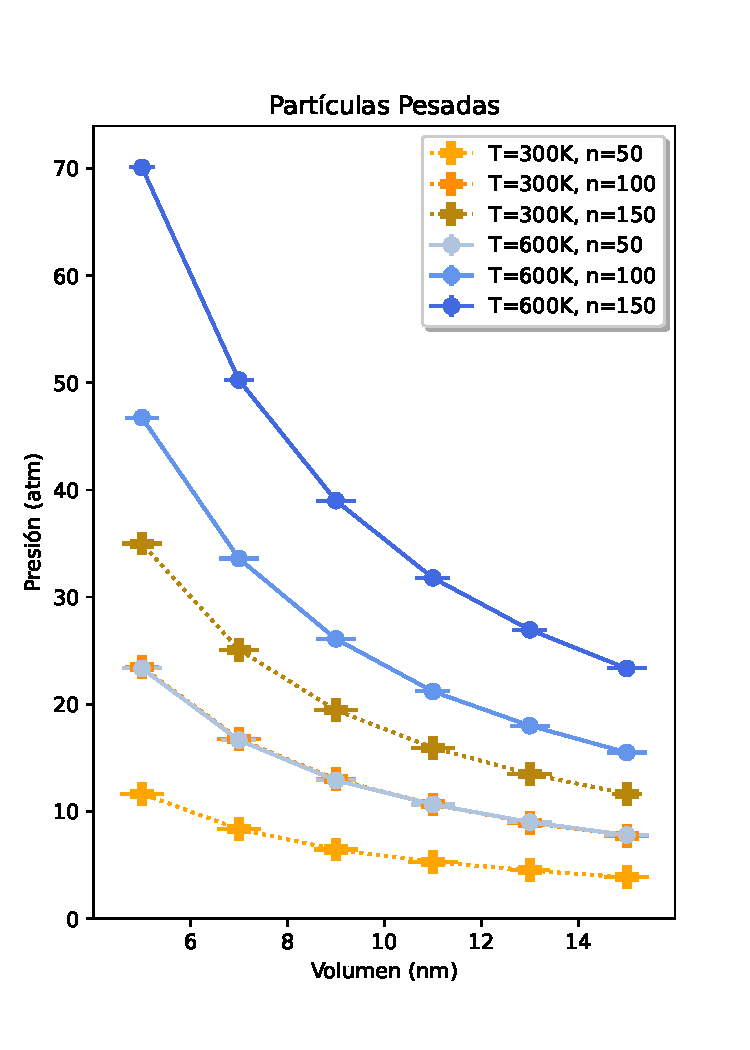
\includegraphics[width=0.5\textwidth]{img/grafico-PP.pdf}
    \caption{Gráfico 1 Partículas Pesadas }
    \label{fig:GPP1}
\end{figure}

\begin{figure}[ht]
    \centering
    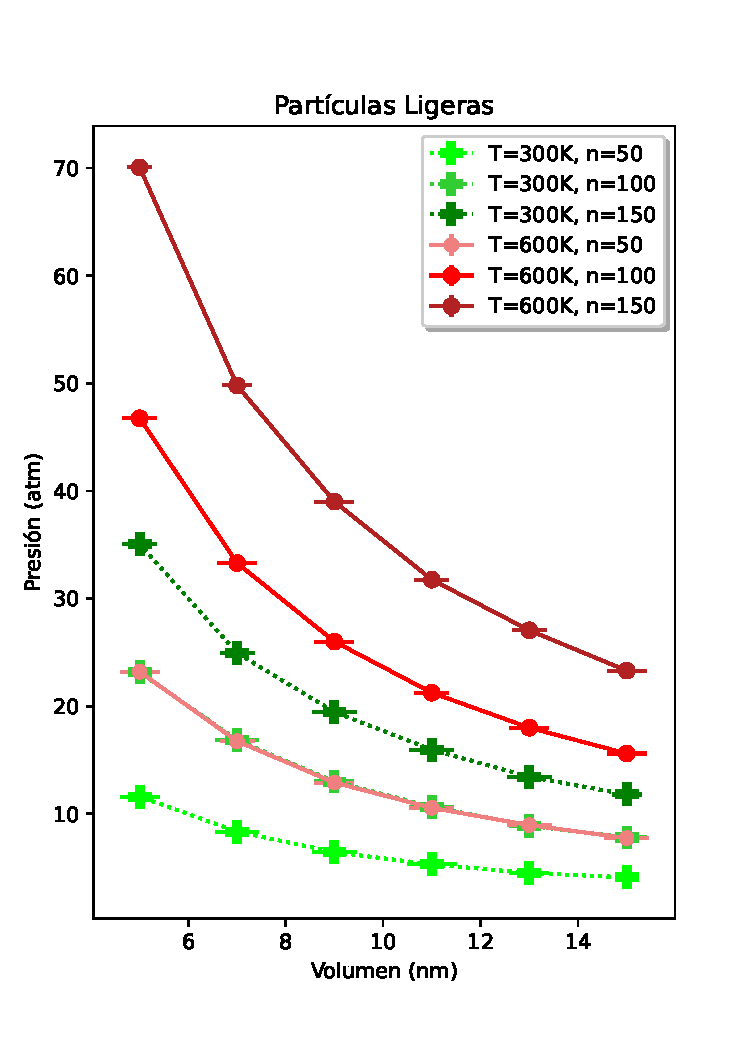
\includegraphics[width=0.5\textwidth]{img/grafico-PL.pdf}
    \caption{Gráfico 1 Partículas Livianas }
    \label{fig:GPL1}
\end{figure}

\begin{figure}[ht]
    \centering
    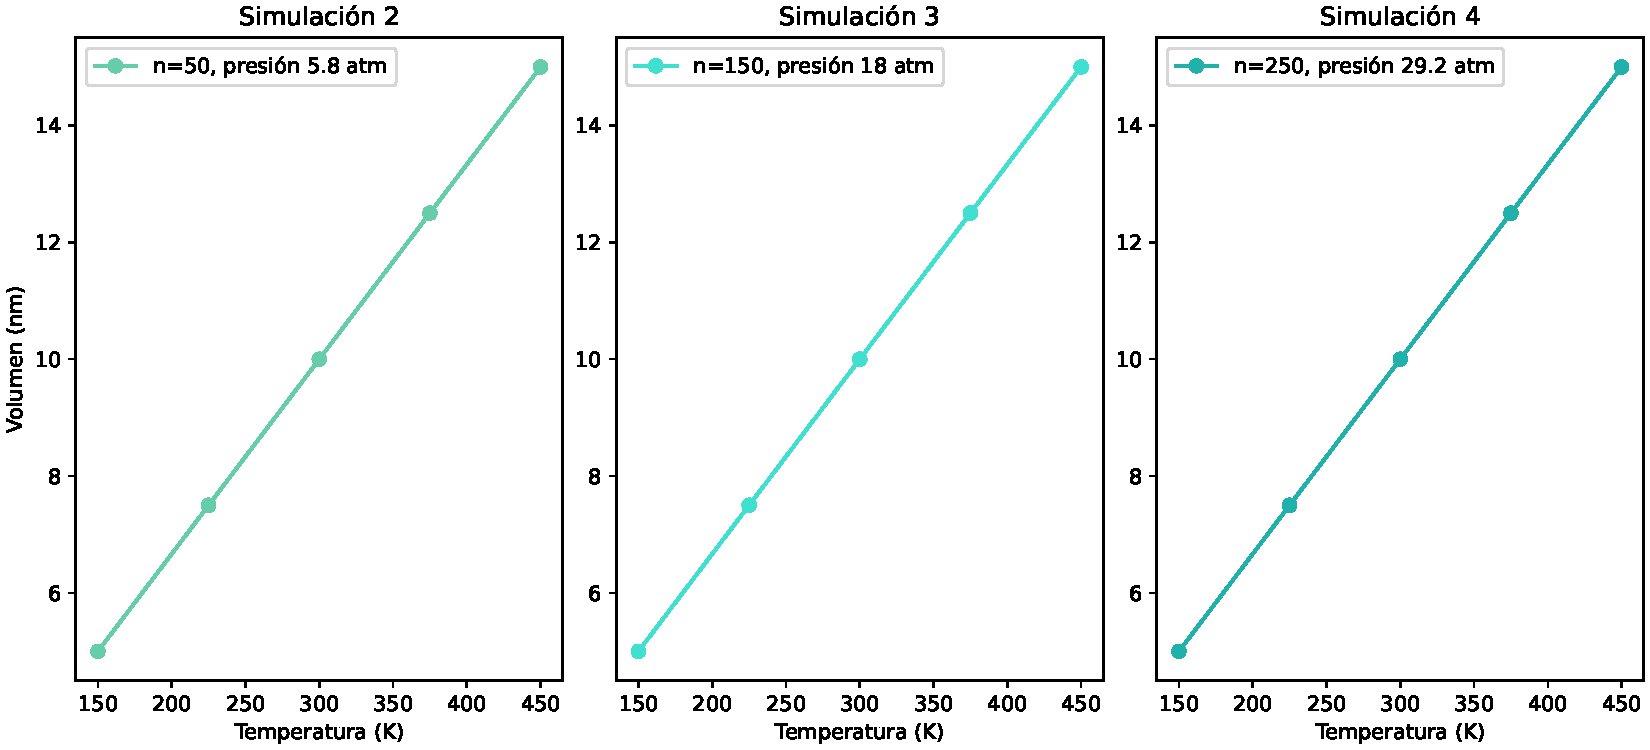
\includegraphics[width=1.0\textwidth]{img/grafico(2,3,4).pdf}
    \caption{Gráficos 2, 3 y 4 }
    \label{fig:GPL1}
\end{figure}

\end{document}
